
\chapter{Background} % Main chapter title

\label{Chapter2} % Change X to a consecutive number; for referencing this chapter elsewhere, use \ref{ChapterX}

%----------------------------------------------------------------------------------------
%	SECTION 1
%----------------------------------------------------------------------------------------
\section{End-to-End Deep Learning Frameworks}

In order to create to run a DL model, a programmer must describe the
architecture, its input and output layers, and the inputs that will be passed
to the model. Beyond these properties, the implementation and challenges
associated with deploying such a model on a DLA or distributed system is
handled by deep learning frameworks. Deep learning frameworks abstract the
implementation and execution details from the programmer such that the
programmer may focus on the model creation only. The abstraction of such
details forces the trade-off of performance and generality as the frameworks
must optimize the same model for runtime and memory efficiency on a diverse set
of available hardware that all have different memory hierarchies, number of PEs,
% TODO: fix this run on
and supported operations. Frameworks must be able to decipher model
descriptions in high level languages such as Python \ref{lst:tensorflow_desc}, apply hardware agnostic
optimizations, and map operations to a specific hardware to create an executable
that will run the model to completion device.

Conventional compilers (eg. Clang) typically take a high level language down to
an intermediate representation (IR) to then machine code that can run on a
device.  The front end is responsible for what parses and lexes the high level
code into a control flow graph, the middle end is responsible for lowering it
to IR and running optimization passes on the IR, and the backend lowers the IR
further into machine code. Similarly, DL frameworks can be broken down into a
front-end, middle-end, and backend. However, there are major differences in the
role of each section and how they are performed.  Deep learning frameworks
deal with a small set of operations that are highly parallelizable but with
variable-sized data \cite{nGraph}. Some operations include: sigmoid, matrix
multiply, vectorsum, L1 Norm, element wise multiply, and dropout among others
\cite{cntk}. Further, a programmer for a given deep learning framework will
work with a domain specific language (DSL) such as Tensorflow
\cite{tensorflow}. Because DSLs only concern with the description of deep
learning networks, the runtime execution, memory, and device management is
managed by the framework. A framework that enables the deployment of a deep
learning model onto hardware from only a high level language description is
called an end to end framework.


\lstinputlisting[language=Python, label={lst:tensorflow_desc}, caption={Python model
description example}, basicstyle=\ttfamily\scriptsize]{Figures/high_level_model_description.py}


\subsection{Graph vs IR based Deep Learning Frameworks}

\begin{figure}[th]
\centering
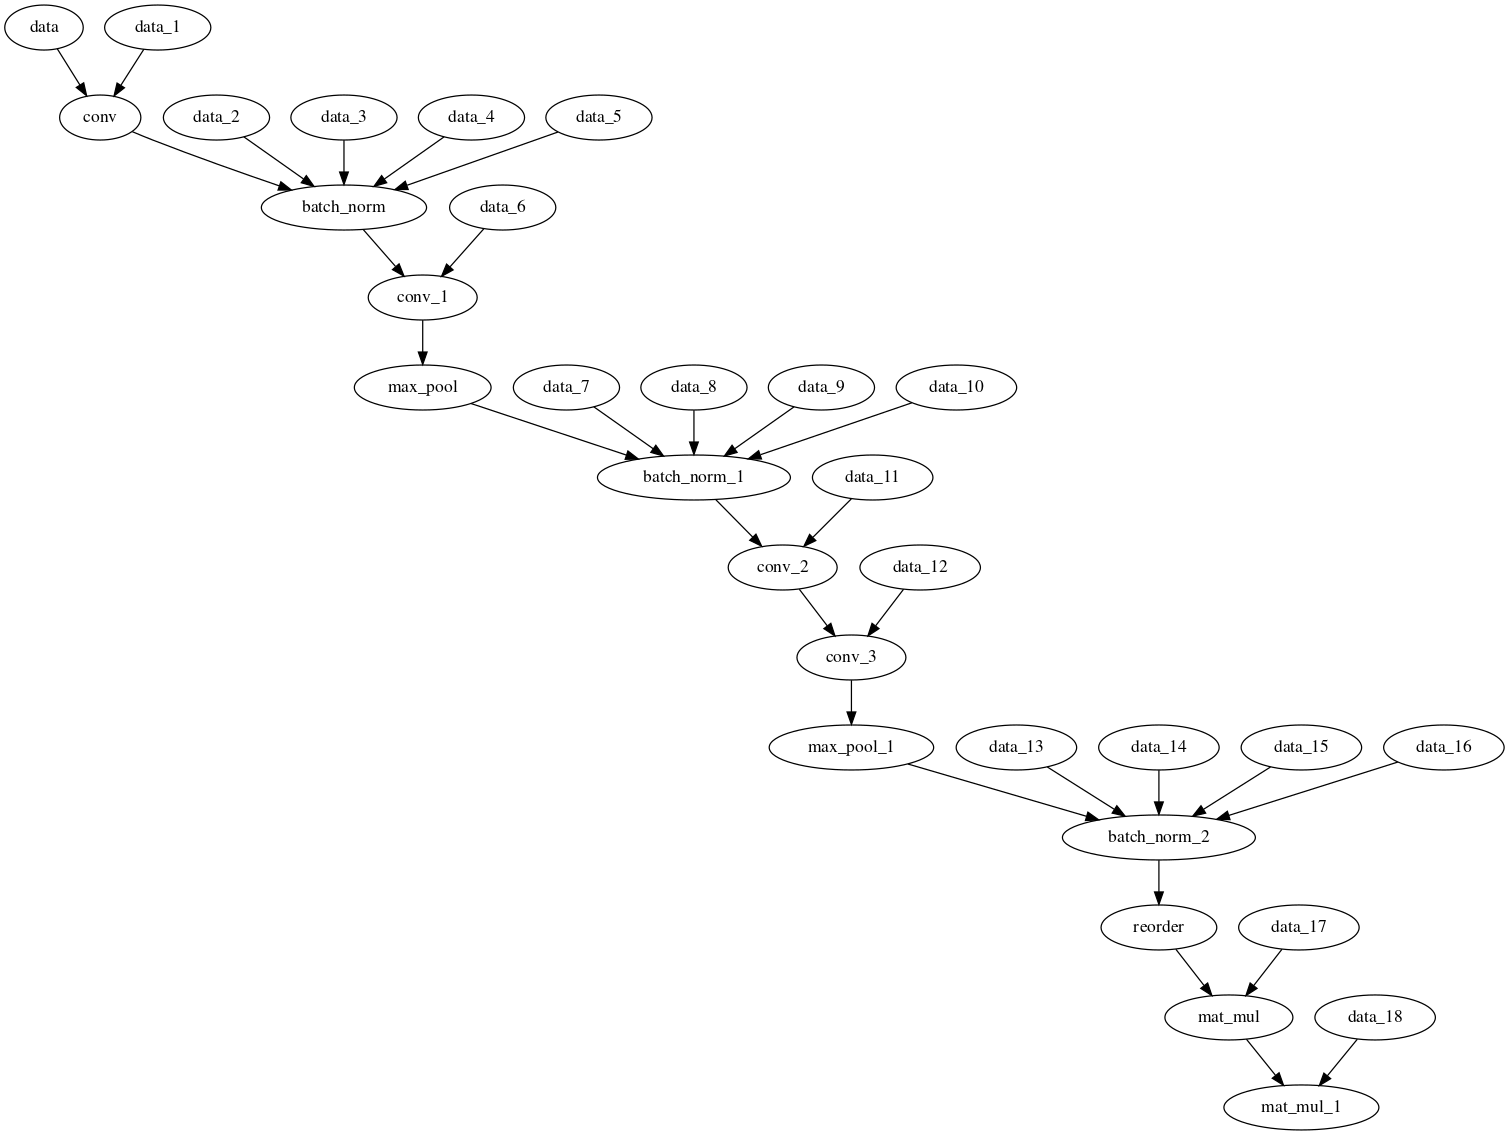
\includegraphics[scale=0.3]{Figures/cnn_smv_dataflow_graph.png}
\decoRule
\caption[cnn]{Computational graph of Cifar-CNN10}
\label{fig:comp_graph_cnn}
\end{figure}

\begin{figure}[th]
\centering
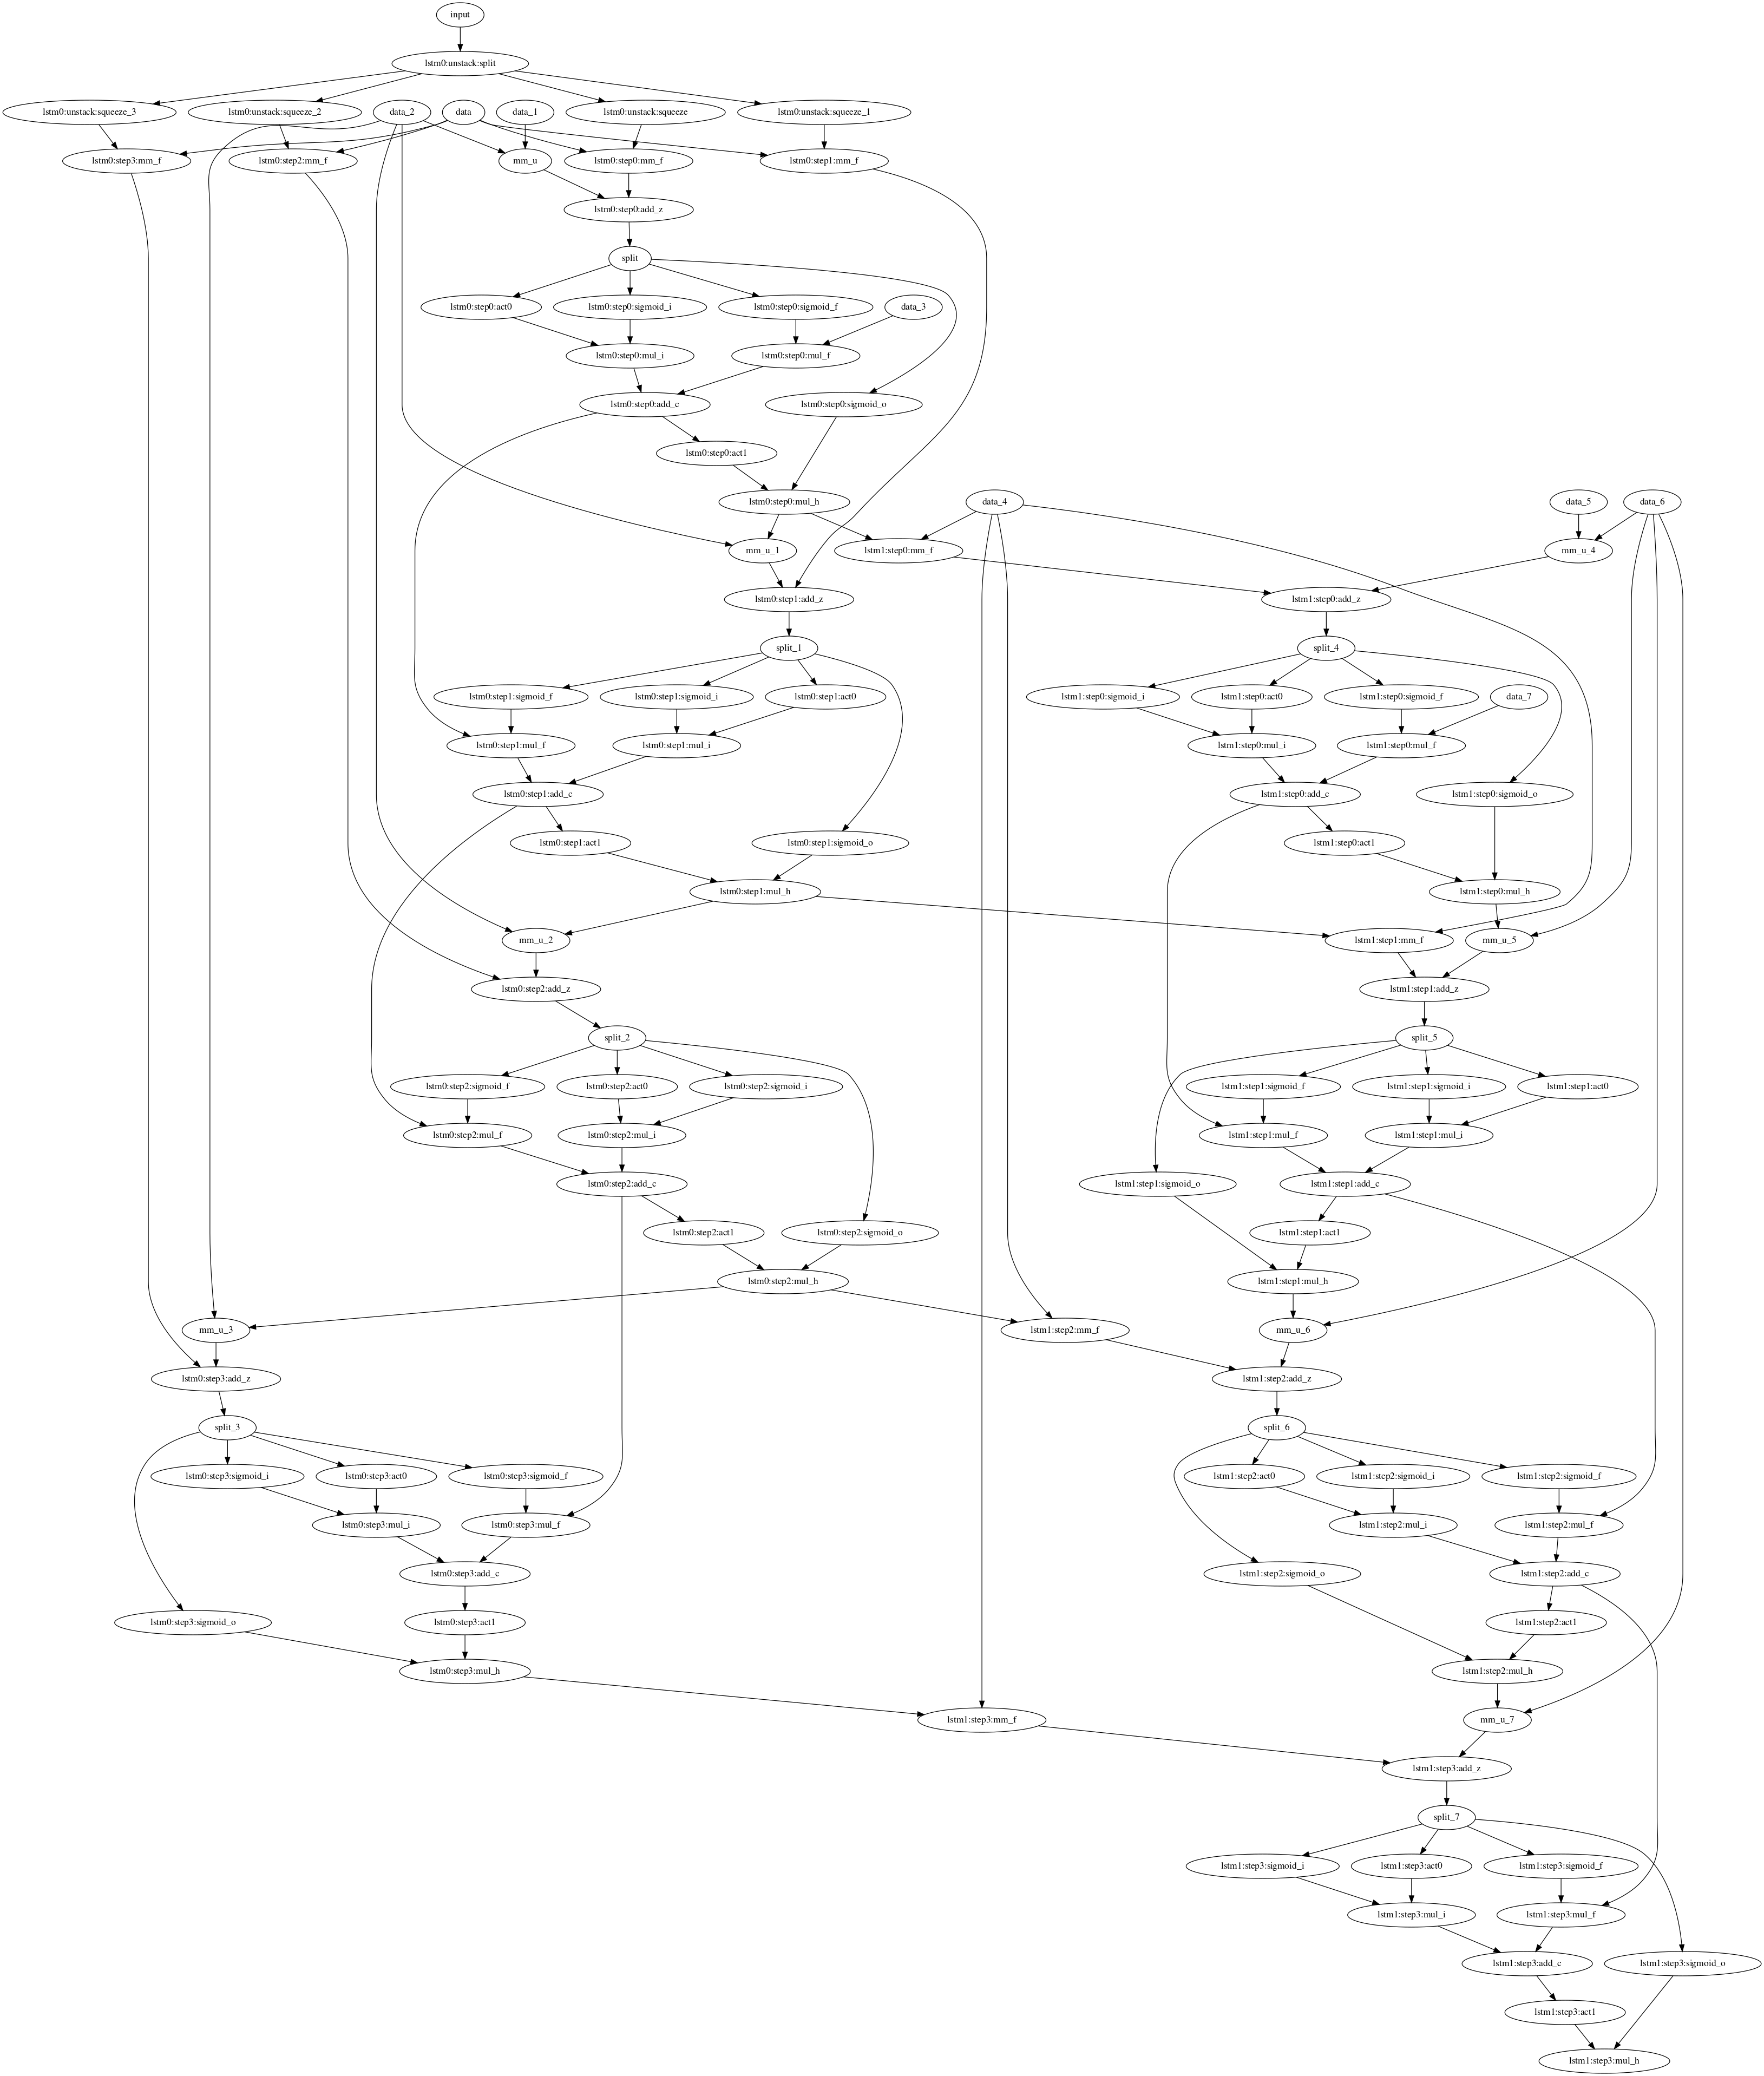
\includegraphics[scale=0.1]{Figures/lstm_dataflow.png}
\decoRule
\caption[lstm]{Computational graph of LSTM}
\label{fig:comp_graph_lstm}
\end{figure}

% TODO: use the toplib explanation of differnt operators that make up a graph
% to explain this part
A common interface used by most DL frameworks is the computational graph
\cite{tensorflow} \cite{cntk} that represents a network of operations needed to
run a DL model. Each DL model can be broken down into a series of discrete
computational operations that can be applied to an input to describe a given
model. A graph made up of vertices and edges where the vertices represent an
operation and the edges represent tensors that flow from one operation to the
next can be used to fully describe a DL model. Computational graphs are
directed acyclic graphs (DAG).  Each vertex can have between zero and two
% TODO: we need to explain how deep leraning models archs look like to describe
% how the concept of layers and "stacking" works to make this explaniation work
% TODO: create a figure of DL computational graph
inputs and zero to one outputs. So for each model, each node in each layer can
be broken down into an operation that maps to a node in the graph. An operation
is a particular computation that must be ran with a set of inputs and outputs.
The implementation of the operation is defined by a kernel. A kernel is
specific to a hardware architecture and are mapped to each operation by the
backend. For example a matrix multiply operation is an essential operation
that reoccurs frequently in computation graphs; the implementation of a matrix
multiply will depend on how many processing elements (PE) the DLA has and its
memory hierarchy. A tensor is a multi-dimensional array that can take on many
types (eg., floating point, int8) and are the inputs and outputs of operations.
Tensors are what are passed along edges of the graph. The dataflow represented
by a graph can be used to infer dependencies and possible optimizations for the
middle-end to apply. Examples of computational graphs are shown in figure
~\ref{fig:comp_graph_cnn} and figure ~\ref{fig:comp_graph_lstm}.

Intermediate representation (IR) is an alternative representation of DL models
for some frameworks such as \cite{DLVM} \cite{nGraph} \cite{ONNX}. For each
framework that uses IR, the framework typically uses its own IR, however
there are tools such as ONNX that attempt to standardize the IR used in
frameworks. 

% TODO: we don't actually describe what IR is and need to make sure to cleraly
% explain what IR is in regular code and that this is an analogue made to
% speciazlie in describing tensor operations
% TODO: make sure to explain what a tensor is
IR in DL frameworks are a language that support linear algebra instructions and
other general purpose instructions (eg., branch, conditional- branch). DL
models are lowered into the framework's IR and a DAG of control flow
\cite{nGraph} can be created where the vertices are operations and edges are
data. This is similar to a computational graph, however, the expressiveness and
modularity that IR provides may lead to more optimization opportunities
\cite{DLVM}. In a computation graph, each kernel can be tuned to maximize its
performance in isolation. Outside of manual kernel turning, performance gains
come from the reordering of schedules and changing the access pattern of
tensors.  In IR based frameworks, the same types of optimizations can be done
to each instruction that maps to a kernel. However, the kernels in IR are not
picked from a set of pre-made kernels in a supported backend, but rather code
generated into LLVM IR or another lower level IR based on the framework. This
% TODO: this is word salad taht means nothing. like you didn't explain
% anything. make it better
allows static analysis to better fuse redundant operations and kernels together
in a more efficient way than sequentially ordering kernels as done in
computational graph based frameworks. Further, different IRs may come with
a wider range of operations that may be supported than the set of operations in
a computational graph that allow the compiler and code generator to manipulate
the DAG in more ways.

Once a DL model is lowered into IR and its optimization passes are done, the IR
is passed into a code generator as backend code or a more supported IR such as
LLVM IR. A transformer will transform the framework IR into code formatted for
a particular backend. There must be a transformer made for every backend. Otherwise,
in the case of LLVM based IR transformations, only backends that support LLVM
IR are able to be used to generate a final binary.
\subsection{Front End}
% TODO: talk more about DSLs and how they are used and why they need to be
% broken up into expressions -> graph 
The front end of frameworks are responsible for breaking down the high level
descriptions of a DL model, typically in Python or C++ \cite{tensorflow}, and
converting them into computation graphs or IR. These lower level abstractions
allow the framework to more easily apply optimizations for memory and runtime
efficiency. 

\subsection{Middle End}
Most optimizations that occur and the engineering focus of end to end
frameworks lie in the middle end. Middle ends must have a diverse set of
backends in mind and be hardware agnostic. In order to achieve this, an IR or
computational graph representation of a DL model is received from the front
end. Once a constructed dataflow graph in either computational graph or IR
form is passed, several passes of static analysis and optimization occur
\cite{TVM} \cite{DLVM} \cite{tensorflow}. Once a completely optimized dataflow
graph is created, it must then be formatted to be compatible to a particular
backend. This can either mean serializing a computational graph into a one
that a backend can read or applying a transform to the optimized IR to generate
code that is compatible with a backend. Backends are vendor specific compilers
that deal with the device level details for kernel implementations and tuning.
Back-ends will support a subset of formats (ie either serialized computational
graphs or a specific IR) and to that end, there must be significant engineering
effort to support a backend for a given middlend. Consequently, most frameworks
only support a handful or backends such as Nvidia's CUDA backend or BLAS for
CPUs. For supported backends, the middlend must be sure to create a final
computational graph or set of IR modules that do not contain operations or
instructions that are not supported by the predefined kernels in the vendor
provided library of a backend \cite{TVM}.

Optimizations in the middle end can be separated into IR specific and
computational graph specific optimizations. For graph level optimizations,
they are typically higher level than kernel tuning and involve graph
restructuring and fusing of subgraphs. Specific optimizations include
re-ordering or scheduling of operators to maximize data reuse
to hide memory transfer latencies, mapping operators to available kernels
for a target DLA, data layout transformations and operator fusion \cite{TVM}.

Operator fusion is the combining of multiple operators into a single operator.
This is helpful because different operators that are distinct from one another
that can otherwise be fused may be scheduled in an unoptimized way or incur
unnecessary memory transfer costs. Every operation requires an input tensor to
be loaded into the accelerator and an output tensor to be produced to be loaded
% TODO: fix this run on
back into main memory. Without explicit data pinning memory management or
caching, or in cases where pinning may not be feasible due to memory size
constraints of the DLA, intermediate values between two operators where the
output of one is the input to the other, may be necessarily transferred back
and forth between main and device memory. By fusing operators together,
the cost of memory transfers due to separated operators are removed.
Further, by fusing operators together, operator code generation can
be optimized as certain intermediate values may not have to be stored or other
computations may be able to be reduced into simpler forms \cite{TVM} \cite{ONNX}.
A disadvantage to this is, fused operations have to either be code generated
where the performance of the kernel is dependant on the quality of the code
generator without any manual tuning or vendor provided libraries must have
pre-defined fused operators that are available to be mapped into the computational
graph. As the number of operators on a network grows, the number of possible
operators that can be fused also grows with it combinatorially \cite{TVM}.
This is exacerbated with the number of supported data layouts, data types, 
and DLA intrinsics. To this end, a large fused operator
cannot be created such that memory transfer costs are fully hidden optimally.

Data layout transformations are the reformatting of how tensors are passed
to a DLA based on the specific memory hierarchy that the DLA has. To exploit
the shape of tensors the DLA best works with, tiling along certain dimensions or
adding reshape operators to change the layout of the tensor in main memory before
sending to the DLA is one way to minimize inference time and is done at the
computational graph level.

Many of the optimizations that apply to computational graphs can also be done
to IR based frameworks. But because they may be lowered into a lower level IR,
more granular and kernel specific optimizations can also be applied before
being passed to the backend. One optimization example is algebraic
simplification and linear algebra fusion \cite{DLVM}. This involves reordering
matrix multiplications and other linear operations into a single matrix
operation. Another example is transforming subexpressions involving multiple
types of operations into a single matrix operation such as a matrix multiply
and an element-wise add \cite{DLVM}.

\subsection{Back End}
A backend is typically not something that is component of a framework
but a vendor provided compiler for a DLA that may be hooked into a compatible
middle end. A backend may support a small set of input formats that describe
a DL model in the form an optimized version of a computational graph or IR.
At this point, all optimizations and transforms that have occurred have
only been applied to the DL model description provided by the programmer.
The backend will be responsible in creating
an execution engine, outputting a compiled executable, and managing
a runtime environment.

A backend like TensorRT \cite{tensorRT} consists of two phases: a build phase
and runtime phase. During the build phase a kernel search is done to map
available kernels to the operators in the dataflow graph that was passed from
the middle end. A serialized version of the graph is then statically analyzed to
be used as context to generate code for the execution context and runtime
engine.  An engine is a representation of the optimized model with a scheduler,
memory manager, a network of operators, their inputs and outputs, and meta data
of input and output tensors such as size and name of the tensors.  During the
runtime phase, an execution context and runtime engine will be instantiated.
The execution context can then be saved to be loaded later or started to run
inference tasks.

Kernels are highly specialized and must be tuned for a DLAs particular memory
hierarchy, data layout, and intrinsics. Kernels are created either via code
generation or supplied by a vendor library. Kernel tuning optimizations are
% TODO: explain what these means probably
handled by the backend.  This includes loop unrolling, caching, loop
reordering, and tiling. An example of what a kernel for a specific operator
looks like is illustrated in figure \ref{fig:OperatorKernel}

\begin{figure}[th]
\centering
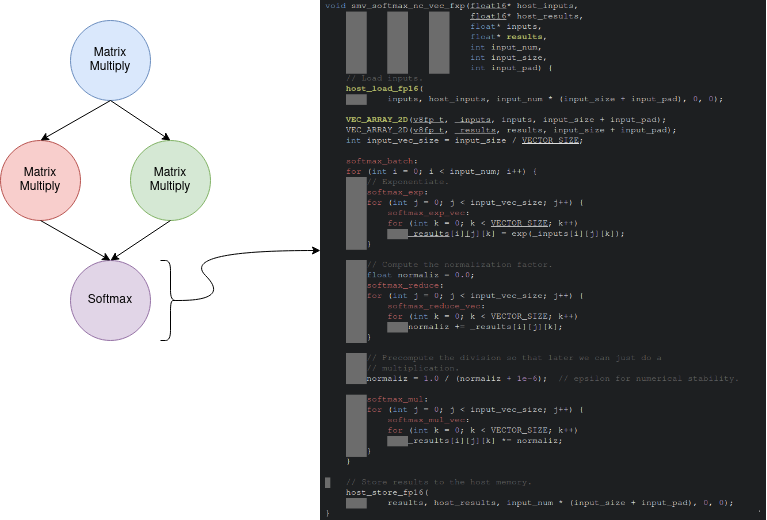
\includegraphics[scale=0.5]{Figures/operator_to_kernel.png}
\decoRule
\caption[operatorKernel]{Estimated \% of data transfers saved for varying scratchpad sizes and models using the optimal pinning strategy}
\label{fig:OperatorKernel}
\end{figure}


\section{Deep Learning Accelerators}

\subsection{Overview of Deep Learning Accelerators}
DNN workloads are made up of millions of
parameters, dozens of different operations that work on multi dimensional data
structures made of thousands of floating point units. However, because of the
finite set of primitive operations that are needed to support the computation
of these models, the repetitive nature of these operations, and type of data
they work with; DL models are highly parallelizable and specialized hardware
can be built to exploit this with maximum efficiency. Some exist to be power
efficient and work in embedded devices while others are made to have no power
constraints so as to maximize compute speed in cloud clusters. In contrast, general
purpose hardware are not able to meet power management needs of many workloads
or cannot compute inference fast enough to meet timing requirements. Examples
of DLAs used are TPUs from Google \cite{tensorflow}, NVDIA's NVDLA \cite{nvdla}, and Intel NNP \cite{nnp}.
An example of an NVDLA based architecture is show in figure \ref{fig:nvdla}.


\begin{figure}[thb!]
\centering
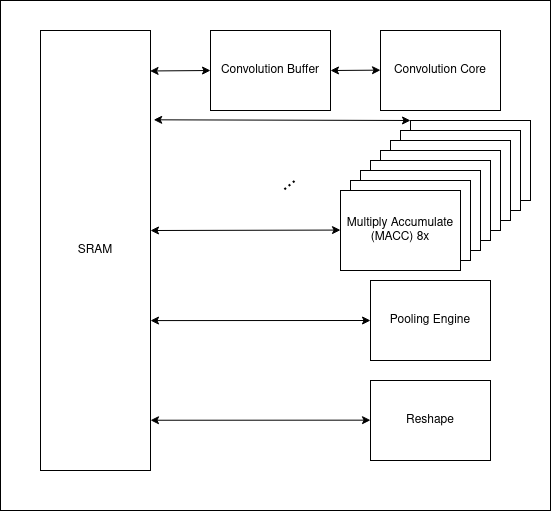
\includegraphics[scale=0.5]{Figures/nvdla.png}
\decoRule
\caption[Reduction]{Architecture of SMAUG's NVDLA-inspired DLA}
\label{fig:nvdla}
\end{figure}


\subsection{Scratchpad Memory}
A key factor that determines the compute and power efficiency of a DLA is how
well its Scratchpad Memory (SPM) is managed. Scratchpad memory is an on-chip
SRAM memory that is managed by software. The transfer of data to and from main
memory must be orchestrated explicitly by the programmer or compiler and the
degree of utilization of the memory is dependant on how it is managed.  This
% TODO: redo this ru non sentence and make it more clear
% TODO: explain better why SPMs are better at repeateable workloads
feature of SPMs is why they have the potential to be more compute and power
efficient than caches due to the predictability of data transfer latencies and
explicit management of data evictions and pinnings without tagging.  Each data
transfer incurs a latency between main and on-chip memory and also power costs
to initiate DMA loads and stores. Caches have hardware that determines when and
what data is transferred but can be unpredictable or unoptimal due to the fact
that eviction and caching schemes are implemented in a heuristic manner
\cite{manyCore}. As a result, SPMs are highly popular for predictable and
repeatable workloads and are used in many embedded devices \cite{graphColoring}
and DLAs \cite{onsram}.


\subsection{Scratchpad Memory Management}
Because SPMs do not contain any hardware logic that deals with pinning and
eviction, all memory transfers between main memory and on-chip-scratchpad-memory
must be explicitly programmed. In workloads where the access patterns are very
predictable or deterministic, this is ideal as the overhead of tag-decoding
logic is avoided and superior performance gains can be had with carefully
optimized memory transfers. Further, software-managed memory leads to more
predictable timing and data transfer costs because of the lack of
tag-decoding logic \cite{graphColoring}. This makes the use of scratchpads
% TODO: we need to explain better intuition of why determinism creates for a
% more highly tuned and optimal management schemes for memory compared to cache
highly desirable for deep learning workloads where the computations and
dataflow are deterministic for any given architecture and therefore the
memory management strategy can be tuned for. Consequently,
the runtime performance of an application is highly dependant on the
ability of a strategy to optimally manage memory and exploit data reuse.

% TODO: epxlain what a kernel is
Scratchpad memory is usually manually programmed by developers
that are specialized in a particular architecture. This is the case for
DLA kernels as well, as most kernels are provided as vendor supplied libraries
where the memory management is optimized \cite{TVM}.

While manual tuning is still used, there exist many limitations that make it
unattractive. Manual tuning requires significant engineering effort, is
vulnerable to bugs, and a strategy is not portable across different
architectures.  Due to these limitations, techniques for compiler based
automated scratchpad memory management have been developed to ease the burden
of programmers. The problem of portability and need for an automated
alternative has been exacerbated for deep learning frameworks and engineers.
The same model could be deployed on several different types of architectures,
each with their own memory hierarchy.  Creating memory optimized operator
schedules, pinning directives, and kernels for each of these architectures is
time consuming and requires specialized knowledge of each architecture. The
implementation of such strategies requires a low level language to describe as
well, which forces a DL engineers who typically work in high level language
frameworks to be an expert in many more fields at once.  While most automated
compiler implementations have been aimed at embedded devices programmed in C
\cite{graphColoring} \cite{memoryColoring}, in recent years there have been
compiler tools built for deep learning workloads as well \cite{onsram}
\cite{toplib}.

The goal of an SPM management strategy is to minimize incurring the cost of
data transfers by maximizing the reuse of data in the SPM. To achieve this,
three main techniques explored in the compiler space: graph coloring, Integer
Linear Programming (ILP), and heuristic based approaches.

Graph coloring for SPMs comes from using graph coloring for the register
allocation problem \cite{registerAllocation} \cite{graphColoring}. A compiler
can decide what variables should be kept in what registers during their
lifetimes and how often they should be swapped between main memory.  The
objective of register allocations are the same as scratchpad management
schemes: to minimize the amount of swaps. This is achieved by constructing
interference graphs of variables whose lifetimes overlap and therefore require
to be placed in separate registers. An interference graph can then be used to
apply a greedy graph coloring algorithm where the number of registers maps to
the number of colors to determine the optimal register allocation scheme.
Scratchpad management can be done by extending this idea where the scratchpad
is partitioned into psuedo-register files \cite{graphColoring}. Applying this
to deep learning workloads is non-trivial as the tensor sizes are variable and
can be larger than the size of the scratchpad. \cite{toplib} discusses graph
coloring implantations for deep learning workloads in the context of maximizing
SPM utilization within kernel code. Figure \ref{fig:graph_color} shows an example
of how TopLib \cite{toplib} uses a graph coloring register allocation strategy
to fit intermediate tensors onto a scratchpad in a kernel.

Similarly, by considering an SPM with fixed size partitions to emulate registers,
an Integer Linear Program (ILP) made to solve the register allocation problem can
be extended to find an optimal strategy for an SPM as discussed in \cite{verma}.

\begin{figure}[thb!]
\centering
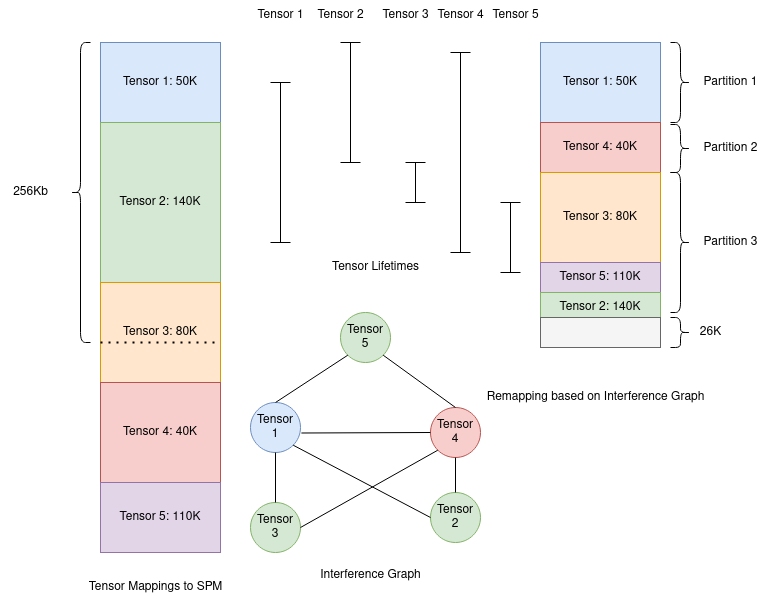
\includegraphics[scale=0.5]{Figures/graph_coloring_example.png}
\decoRule
\caption[graphColoring]{Example of graph coloring. Not all tensors can be
mapped to the SPM at the same time so an interference graph is created
based on their lifetimes and colored accordingly. The resulting mapping on the 
right contains partitions for tensors based on their lifetime and colors such that
all tensors fit on the SPM without contention.}
\label{fig:graph_color}
\end{figure}
%----------------------------------------------------------------------------------------
%	SECTION 2
%----------------------------------------------------------------------------------------
% TODO: explain DL workloads better: why they're parallelizable ; why consumer
% hardware sucks
% TODO: need more backgroudn on what DLAs look like and how they are superior to DL
% Workloads so that later on when we describe operators in graphs and why
% kernels are differnt for every arch it makes sense and we can also smoothly
% talk about why DL compilers need so many backends since there is no
% standardized IR



% TODO: algorthim of a one hiddle layer sigmoid like in CNTK

% TODO: figure of DAG -> operation -> kernel code snippet

% TODO: figure of Matrix operations -> DAG -> kernel code

% TODO: figure of NN -> DAG


%IR

% TODO: Figure of DL arch -> IR -> IR CFG

%Front end
%middle end

%backend
